\documentclass[tikz,border=10pt]{standalone}
\usetikzlibrary{shapes.misc}

\begin{document}
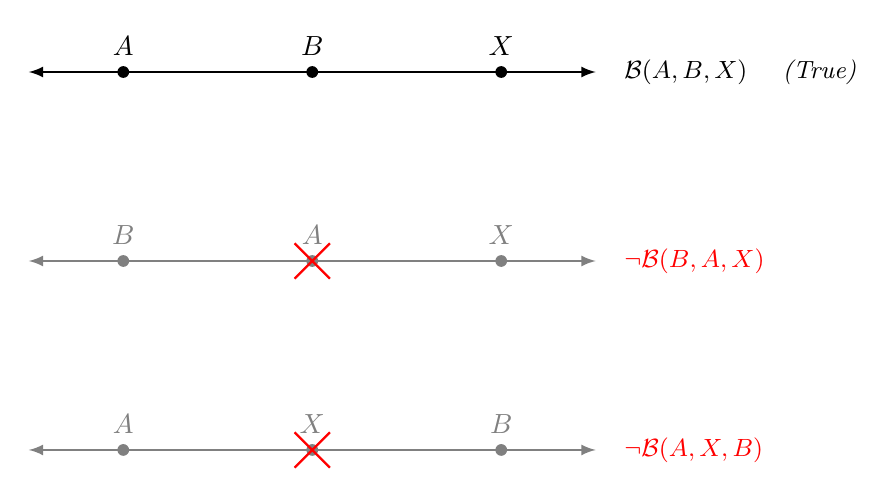
\begin{tikzpicture}[>=stealth, scale=1.2]

  % Styles
  \tikzset{
    point/.style={circle, fill=black, inner sep=1.5pt},
    label style/.style={font=\small, fill=white, inner sep=2pt},
    cross/.style={cross out, draw=red, thick, minimum size=12pt, inner sep=0pt}
  }

  % --- CONFIGURATION 1: B is between A and X (TRUE) ---
  \begin{scope}[shift={(0,2)}]
    % Line
    \draw[latex-latex, thick] (-1,0) -- (5,0);
    % Points
    \node[point, label=above:$A$] (A1) at (0,0) {};
    \node[point, label=above:$B$] (B1) at (2,0) {};
    \node[point, label=above:$X$] (X1) at (4,0) {};
    % Label
    \node[right, font=\small\itshape] at (5.2,0) {$\mathcal{B}(A,B,X)$ \quad(True)};
  \end{scope}

  % --- CONFIGURATION 2: A is between B and X (IMPOSSIBLE) ---
  \begin{scope}[shift={(0,0)}]
    % Line
    \draw[latex-latex, thick, gray] (-1,0) -- (5,0);
    % Points
    \node[point, gray, label=above:\color{gray}$B$] (B2) at (0,0) {};
    \node[point, gray, label=above:\color{gray}$A$] (A2) at (2,0) {};
    \node[point, gray, label=above:\color{gray}$X$] (X2) at (4,0) {};
    % Cross-out indicating impossibility
    \node[cross] at (2,0) {};
    % Label
    \node[right, font=\small\itshape, red] at (5.2,0) {$\neg\mathcal{B}(B,A,X)$};
  \end{scope}

  % --- CONFIGURATION 3: X is between A and B (IMPOSSIBLE) ---
  \begin{scope}[shift={(0,-2)}]
    % Line
    \draw[latex-latex, thick, gray] (-1,0) -- (5,0);
    % Points
    \node[point, gray, label=above:\color{gray}$A$] (A3) at (0,0) {};
    \node[point, gray, label=above:\color{gray}$X$] (X3) at (2,0) {};
    \node[point, gray, label=above:\color{gray}$B$] (B3) at (4,0) {};
    % Cross-out indicating impossibility
    \node[cross] at (2,0) {};
    % Label
    \node[right, font=\small\itshape, red] at (5.2,0) {$\neg\mathcal{B}(A,X,B)$};
  \end{scope}

\end{tikzpicture}
\end{document}
